% preamble and style file for M&R lecture slides
\documentclass[11.5pt,sans,english]{beamer}

\usetheme{EastLansing}
\usecolortheme{lily}

\usepackage[most]{tcolorbox}

\usepackage{verbatim}
%\usepackage{ulem}
%\usepackage{fontawesome}
%\usepackage{tikz}
%\usepackage{pifont}
%\usepackage{tabularx}
\usepackage{array,booktabs,xcolor,colortbl,multirow,rotating,amssymb}
%\usepackage{amsmath}
% \usepackage{vwcol}
% \usepackage[T1]{fontenc}

  
\newcommand\vect[1]{\underline{\mathbf{#1}}}
\newcommand\unitvect[1]{\hat{\boldsymbol{#1}}}
%\newcommand\hatdot[1] { \hat{ \dot{ \boldsymbol{#1} } } }

\newtcbox
{\keyc}{on line,arc=2pt, colback=yellow!30!white, colframe=yellow!30!black, before upper={\rule[-3pt]{0pt}{10pt} },boxrule=1pt,boxsep=0pt,left=6pt,right=6pt,top=2pt,bottom=2pt,}

\newtcbox
{\keyb}{on line,arc=1pt, colback=blue!30!white, colframe=blue!30!black, before upper={\rule[-3pt]{0pt}{10pt} },boxrule=1pt,boxsep=0pt,left=6pt,right=6pt,top=2pt,bottom=2pt,}

\newtcbox
{\keyl}{on line,arc=1pt, colback=pink!30!white, colframe=blue!30!black, before upper={\rule[-3pt]{0pt}{10pt} },boxrule=1pt,boxsep=0pt,left=6pt,right=6pt,top=2pt,bottom=2pt,}

\newtcbox
{\keyw}{on line,arc=1pt, colback=red!30!white, colframe=blue!30!black, before upper={\rule[-3pt]{0pt}{10pt} },boxrule=1pt,boxsep=0pt,left=6pt,right=6pt,top=2pt,bottom=2pt,}

\newtcbox
{\keya}{on line,arc=1pt, colback=purple!30!white, colframe=blue!30!black, before upper={\rule[-3pt]{0pt}{10pt} },boxrule=1pt,boxsep=0pt,left=6pt,right=6pt,top=2pt,bottom=2pt,}

\newtcbox[auto counter,number within=section]
{keyf}
{
enhanced,
on line,
  boxsep=0pt,
  left=6pt,right=6pt,top=2pt,bottom=2pt,
  arc=5pt,
  boxrule=1pt,
  rightrule=38pt,
colback=green!10!white, 
colframe=green!50!black, 
title=\thetcbcounter,
detach title,
overlay unbroken and first ={
    \node[%rotate=90,
          %minimum width=1cm,
          anchor=south,
          font=\sffamily\bfseries\tiny,
          %yshift=-10pt,
          yshift=-5pt,
          xshift=-20pt,
          white]
    at (frame.east) {\thetcbcounter};
  }
}


\usepackage{xcolor}

%\usepackage{hyperref}
%\hypersetup{
%  pdfauthor={Lily Asquith},
%  urlcolor=blue,
%  colorlinks=true,
%  linkcolor=blue,
%  bookmarks=true
%}

%---------------------------------------------%
%              LILY'S COLOURS           %
%---------------------------------------------%
\definecolor{Wash}{RGB}{204,204,204}
%\definecolor{Pinky}{RGB}{254,200,254}%violet
\definecolor{Pinky}{RGB}{219,	240,	253}%violet
\definecolor{Bluey}{RGB}{0,190,255}%deep sky blue
\definecolor{DarkGrey}{RGB}{28,66,137}%dar grey
\definecolor{SussexWhite}{RGB}{253,255,254}%dar grey
\definecolor{LightGray}{RGB}{184,184,255}
\definecolor{YesGreen}{RGB}{0,128,0}
\definecolor{NoRed}{RGB}{250,0,0}



\definecolor{myred}{RGB}{255,153,153}
\definecolor{myorange}{RGB}{255,204,153}
\definecolor{myyellow}{RGB}{255,255,153}
\definecolor{mygreen}{RGB}{153,255,153}
\definecolor{mycyan}{RGB}{153,255,255}
\definecolor{myblue}{RGB}{153,204,255}
\definecolor{myviolet}{RGB}{153,153,255}
\definecolor{mypurple}{RGB}{204,153,255}
\definecolor{mypink}{RGB}{255,204,255}
\definecolor{mycoral}{RGB}{255,153,204}

%-----------------------------------------------------%
%              LILY'S COLUMN TYPES          %
%-----------------------------------------------------%
\newcolumntype{a}{>{\raggedright\arraybackslash}l}	
\newcolumntype{q}{>{\raggedright\arraybackslash}m{8cm}} 

%--------------------------------------------%
%              LILY'S SYMBOLS          %
%--------------------------------------------%
\newcommand{\dfinger}{\large{\textcolor{black}{\ding{43}}}\scriptsize}
\newcommand{\dstar}{\large{\textcolor{black}{\ding{76}}}\scriptsize}
\newcommand{\dwrite}{\large{\textcolor{black}{\ding{45}}}\scriptsize}
\newcommand{\ddiamond}{\small{\textcolor{DarkGrey}{\ding{117}}}\scriptsize}
\newcommand{\ddiamondwhite}{\small{\textcolor{SussexWhite}{\ding{117}}}\scriptsize}
\newcommand{\experiment}{\small{\textcolor{magenta}{\faCogs }}\scriptsize}
\newcommand{\watchit}{\textcolor{blue}{ \faYoutube}}


\makeatletter
\newcommand\notsotiny{\@setfontsize\notsotiny{6.5}{7.5}}
\makeatother


% 
\title[ Mechanics \& Relativity]{Mechanics \& Relativity}
%\subtitle{\textbf{Topic 1: Kinematics }}
\author[Dr Lily Asquith (Lily)]{ Dr Lily Asquith (Lily)}
\date[Week 7 ]{Week 7 }
\logo{

\includegraphics[width=1.5cm]{../../utils/uslogo.jpg}
}


\begin{document}


\begin{frame}
\titlepage
\end{frame} 

 \subsection{ Familiar Angular Variables}
 
\begin{frame}{Familiar Angular Variables}
\small

Angular displacement: $\theta  = \frac{s}{r}$\\[2ex]
Angular velocity: $\omega  = \frac{d\theta}{dt} = \frac{1}{r} \frac{ds}{dt} = \frac{v}{r}$\\[2ex]
Angular (Tangential) acceleration: $\alpha  = \frac{d\omega}{dt} = \frac{1}{r} \frac{d^2s}{dt^2} = \frac{a}{r}$\\[2ex]
Angular (Radial) acceleration: $a_c  = - \frac{v^2}{r}$\\[2ex]
Period: $T = \frac{s}{v} = \frac{\theta}{\omega} = \frac{2\pi}{\omega}$\\[2ex]

\end{frame}

\begin{frame}{Familiar Angular Variables}
\small
The angular position of a point on a rotating wheel is given by\\[1ex]
 $\theta$ = 2.0 [rad] + 4.0 [rad s$^{-2}] t^2$ + 2.0 [rad s$^{-3}] t^3$.\\[2ex]
(a) At t = 0, what is the point's angular position? \\[1ex]
(b) At t = 0, what is its angular velocity? \\[5ex]
(c) What is its angular velocity at t = 4.0 s? \\[1ex]
(d) Calculate its angular acceleration at t = 2.0 s. \\[5ex]
(e) Is its angular acceleration constant?\\[1ex]
\vspace{5cm}
\end{frame}

\begin{frame}{Angular suvat}
\small
For constant angular (tangential) acceleration $\alpha =\frac{a}{r}$:\\[2ex]
$v = u + at \rightarrow \omega = \omega_0 + \alpha t $\\[2ex]
$s = ut + \frac{1}{2}at^2 \rightarrow \theta = \omega_0 t + \frac{1}{2}\alpha t^2 $\\[2ex]
\end{frame}

\begin{frame}{Angular suvat}
\small
The angular speed $\alpha$ of an automobile engine is increased at a constant rate from 1200 rev/min to 3000 rev/min in 12 s.\\[1ex]
 (a) What is its angular acceleration in revolutions per minute-squared?\\[1ex]
 (b) How many revolutions does the engine make during this 12 s interval?\\[1ex]
\end{frame}


 \subsection{ New  Angular Variables}

\begin{frame}{New Angular Variables}
\small
Rotational Inertia (angular mass): $I = \int r^2 dm$\\[1ex]
Torque (angular force): $\tau = r \times F = I\alpha$\\[1ex]
Rotational Work : $W = \int  \tau d\theta$\\[1ex]
Rotational KE : $KE = \frac{1}{2}I\omega^2$\\[1ex]
Angular momentum : $L = r \times p$\\[1ex]
\end{frame}


 \subsection{Inertia \& Torque}
 
 \begin{frame}{Rotational Inertia}
\small
Rotational Inertia (angular mass): $I = \int r^2 dm$\\[1ex]
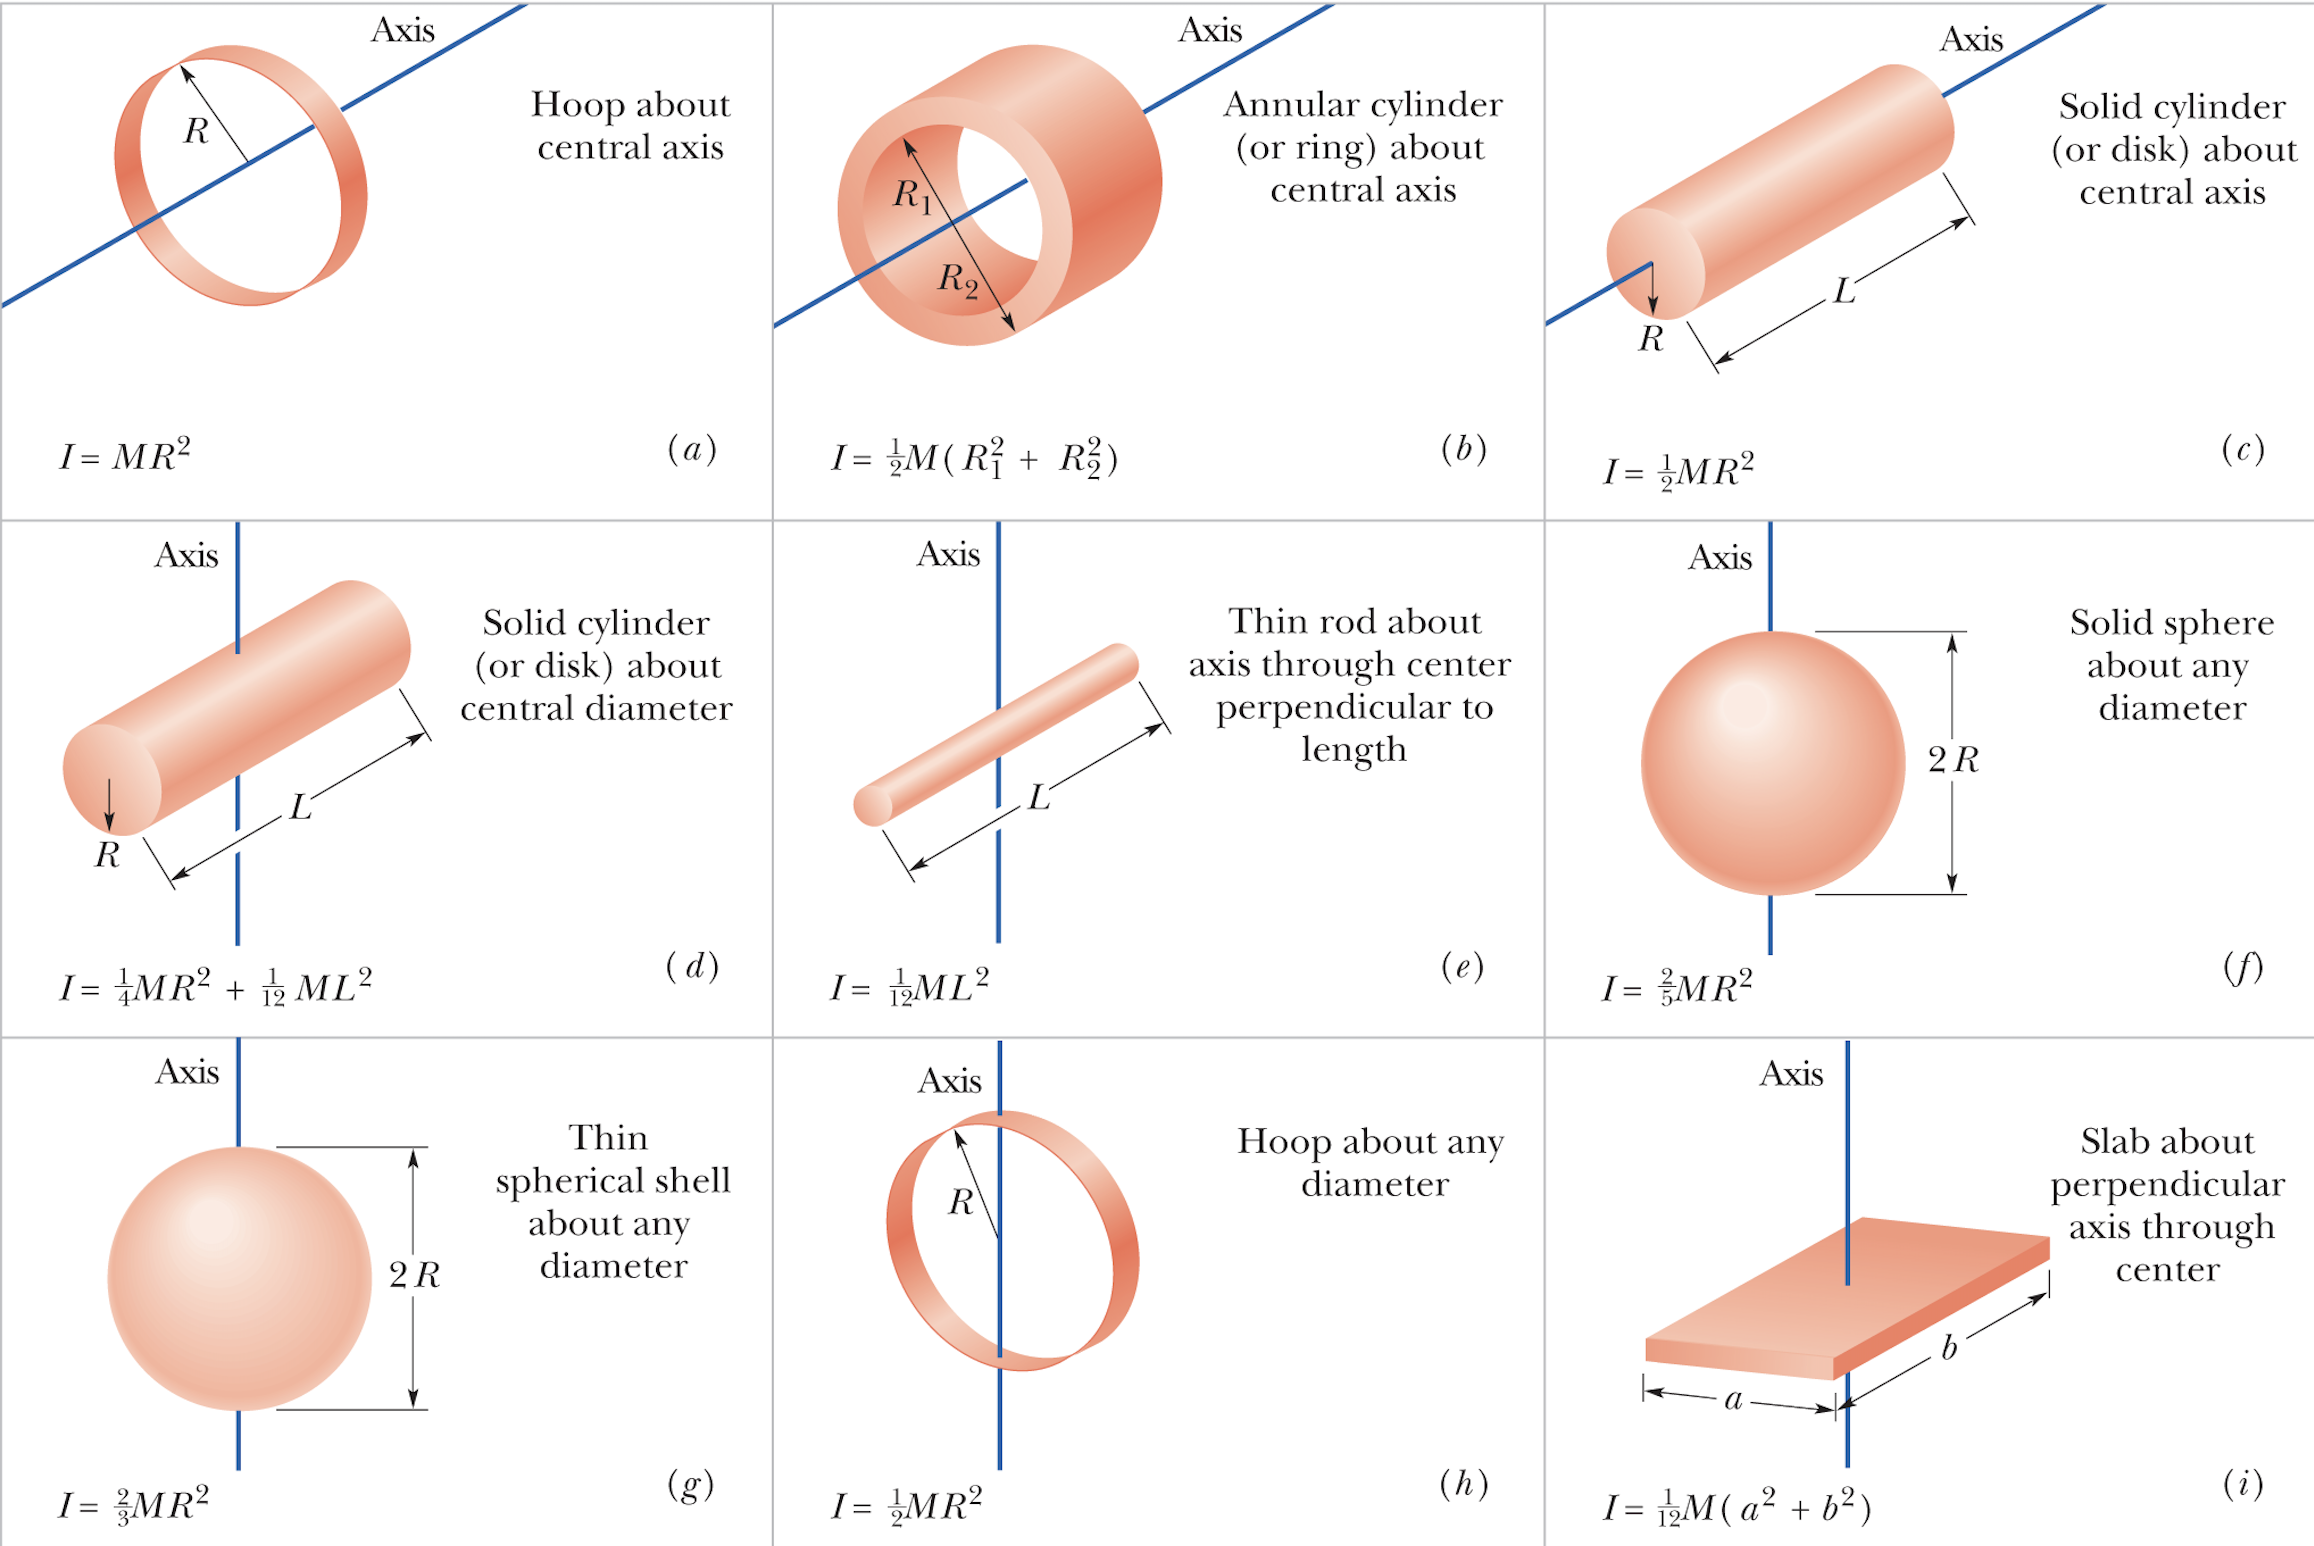
\includegraphics[scale=0.2]{momsofI}
\end{frame}


\begin{frame}{Torque}
\small
Torque (angular force): $\tau = r \times F = I\alpha$\\[1ex]
The length of a bicycle pedal arm is 0.152 m, and a downward force of 111 N is applied to the pedal by the rider. What is the magnitude of the torque about the pedal arm's pivot when the arm is at angle \\
(a) 30$^{\circ}$\\[1ex]
 (b) 90$^{\circ}$\\[1ex]
 (c) 180$^{\circ}$ with the vertical?\\[1ex]
\end{frame}

\begin{frame}{Rotational KE}
\small
Rotational KE : $KE = \frac{1}{2}I\omega^2$\\[1ex]
A thin rod of length 0.75 m and mass 0.42 kg is suspended freely from one end. It is pulled to one side and then allowed to swing like a pendulum, passing through its lowest position with angular speed 4.0 rad/s. Neglecting friction and air resistance, find (a) the rod's kinetic energy at its lowest position and (b) how far above that position the center of mass rises.
\end{frame}



 \subsection{Rolling}
 
\begin{frame}{Rolling: translational KE}
\small
We have KE due to the translational movement of the centre of mass of the rolling object: $KE_{tran} = \frac{1}{2}mv_{com}^2$\\[1ex]
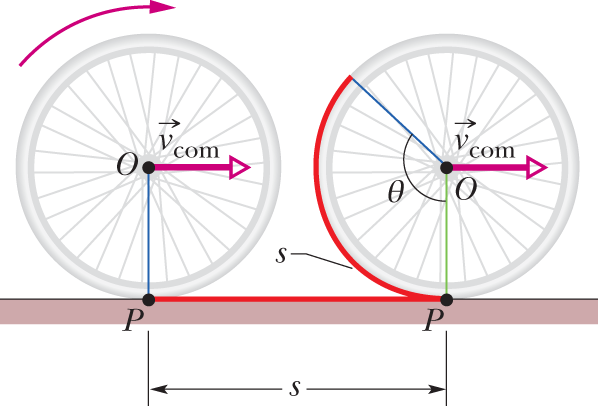
\includegraphics[scale=1]{vcom}
\end{frame}

   \begin{frame}{Rolling: rotational + translational}
\small
We also have KE due to the  rotational movement of the centre of mass of the rolling object: \\[1ex]

$KE_{tot} = KE_{tran} + KE_{rot} = \frac{1}{2}mv_{com}^2 + \frac{1}{2} I \omega^2$\\[1ex]

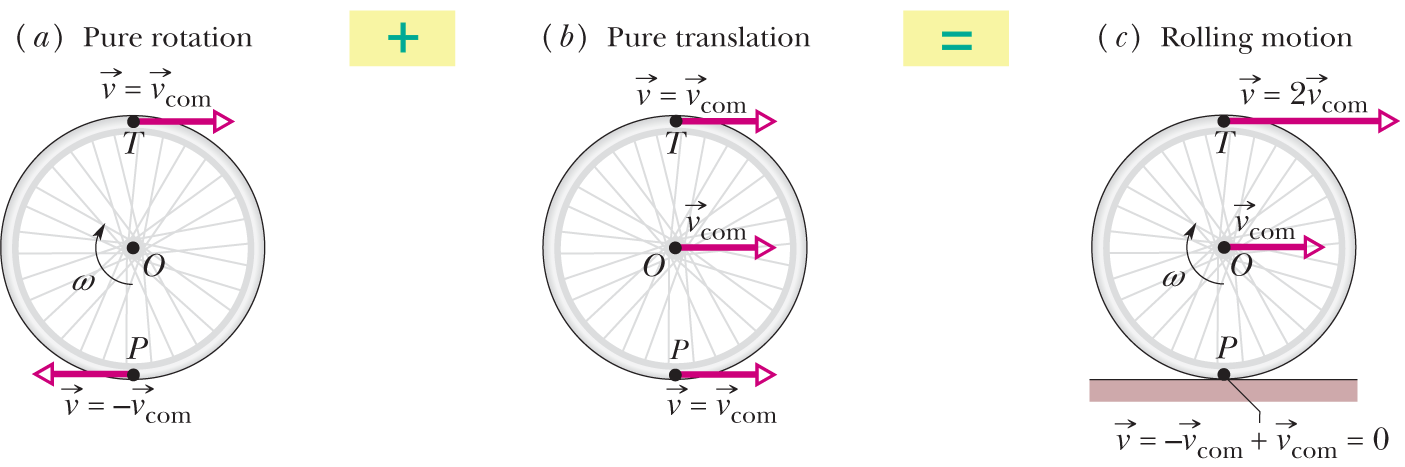
\includegraphics[scale=1]{roll}
\end{frame}

  \begin{frame}{Rolling}
\small

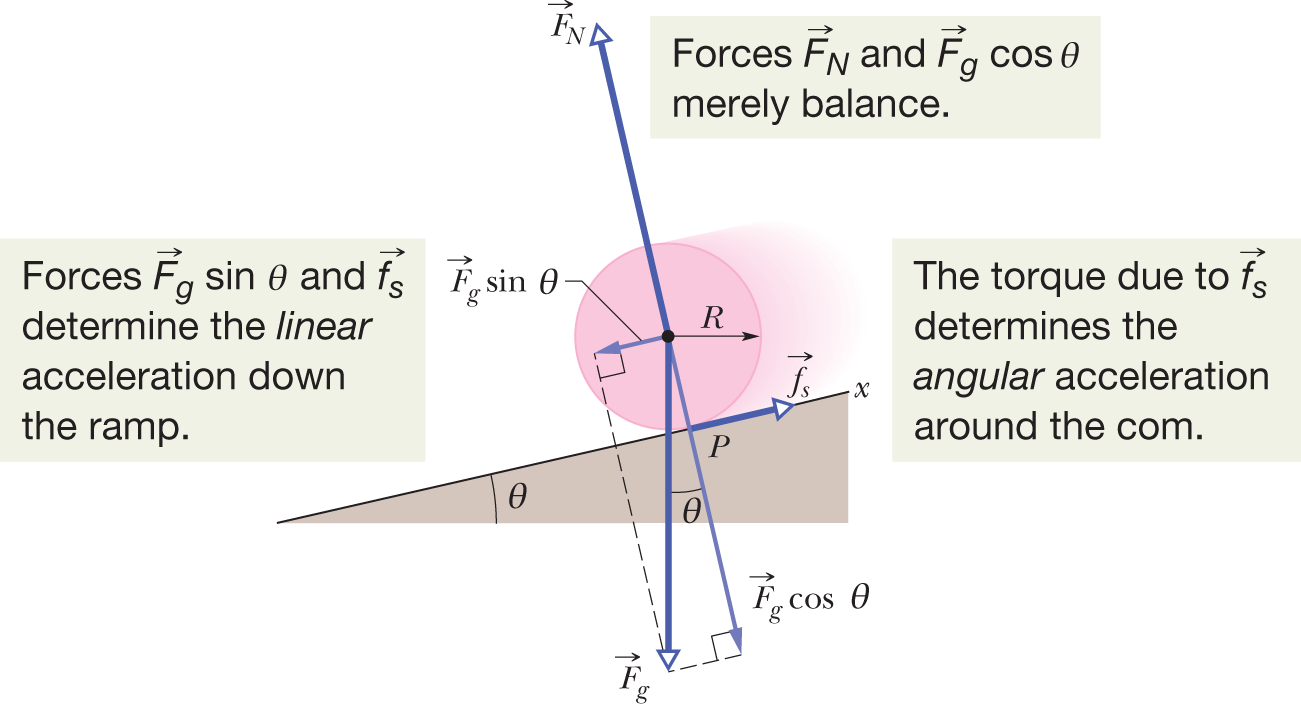
\includegraphics[scale=1]{roll-fric}
\end{frame}


  \begin{frame}{Angular Acceleration Problem}
\small
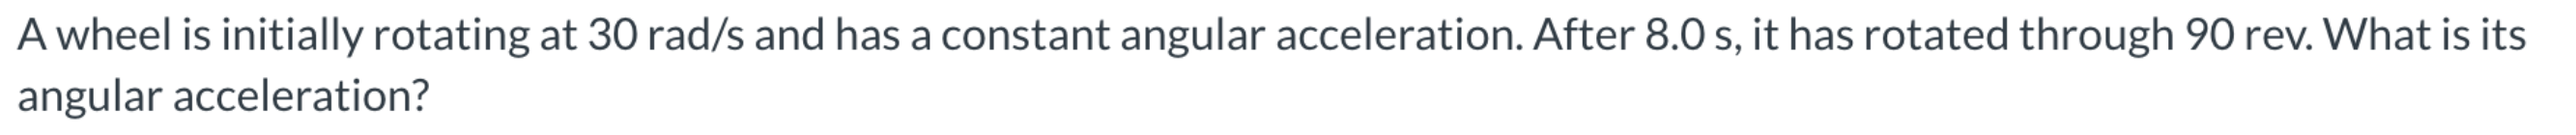
\includegraphics[scale=0.25]{agpro}
\end{frame}



  \begin{frame}{Rolling Problem}
\small
A car traveling at 80.0 km/h has tires of 75.0 cm diameter. \\[1ex]
(a) What is the angular speed of the tires about their axles?\\[1ex]
(b) If the car is brought to a stop uniformly in 30.0 complete turns of the tires (without skidding), what is the magnitude of the angular acceleration of the wheels? \\[1ex]
(c) How far does the car move during the braking?\\[1ex]
\end{frame}

  \begin{frame}{Rolling Problem}
\small
A solid cylinder of radius 10 cm and mass 12 kg starts from rest and rolls without slipping a distance L = 6.0 m down a roof that is inclined at angle $\theta = 30^{\circ}$.\\[1ex]
 (a) What is the angular speed of the cylinder about its centre as it leaves the roof? \\[1ex]
 (b) The roof's edge is at height H = 5.0 m. How far horizontally from the roof's edge does the cylinder hit the level ground?\\[1ex]

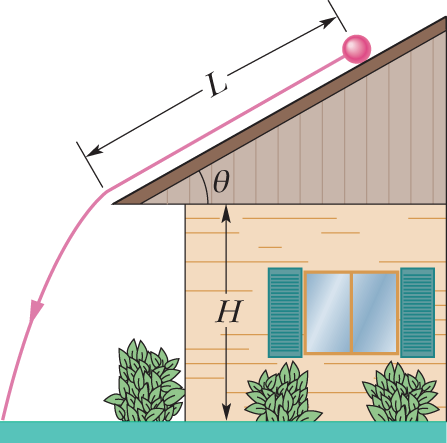
\includegraphics[scale=0.8]{roof}
\end{frame}


 \subsection{ Angular Momentum}
 
   \begin{frame}{Angular Momentum }
\small
Angular momentum : $L = r \times p$\\[1ex]
\end{frame}



  \begin{frame}{Angular Momentum Problem}
\small
A 2.0 kg particle-like object moves in a plane with velocity components $v_x = 30$ ms$^{-1}$ and $v_y = 60$ ms$^{-1}$ as it passes through the point with (x, y) coordinates of (3.0, -4.0) m. Just then, in unit-vector notation, what is its angular momentum relative to \\[1ex]
(a) the origin and \\[1ex]
(b) the point located at (-2.0, -2.0) m?\\[1ex]
\end{frame}
\end{document}